%%
%% Copyright 2022 OXFORD UNIVERSITY PRESS
%%
%% This file is part of the 'oup-authoring-template Bundle'.
%% ---------------------------------------------
%%
%% It may be distributed under the conditions of the LaTeX Project Public
%% License, either version 1.2 of this license or (at your option) any
%% later version.  The latest version of this license is in
%%    http://www.latex-project.org/lppl.txt
%% and version 1.2 or later is part of all distributions of LaTeX
%% version 1999/12/01 or later.
%%
%% The list of all files belonging to the 'oup-authoring-template Bundle' is
%% given in the file `manifest.txt'.
%%
%% Template article for OXFORD UNIVERSITY PRESS's document class `oup-authoring-template'
%% with bibliographic references
%%

%%%CONTEMPORARY%%%
%\documentclass[unnumsec,webpdf,contemporary,large]{oup-authoring-template}%
%\documentclass[unnumsec,webpdf,contemporary,large,namedate]{oup-authoring-template}% uncomment this line for author year citations and comment the above
%\documentclass[unnumsec,webpdf,contemporary,medium]{oup-authoring-template}
%\documentclass[unnumsec,webpdf,contemporary,small]{oup-authoring-template}

%%%MODERN%%%
%\documentclass[unnumsec,webpdf,modern,large]{oup-authoring-template}
\documentclass[unnumsec,webpdf,modern,large,namedate]{oup-authoring-template}% uncomment this line for author year citations and comment the above
%\documentclass[unnumsec,webpdf,modern,medium]{oup-authoring-template}
%\documentclass[unnumsec,webpdf,modern,small]{oup-authoring-template}

%%%TRADITIONAL%%%
%\documentclass[unnumsec,webpdf,traditional,large]{oup-authoring-template}
%\documentclass[unnumsec,webpdf,traditional,large,namedate]{oup-authoring-template}% uncomment this line for author year citations and comment the above
%\documentclass[unnumsec,namedate,webpdf,traditional,medium]{oup-authoring-template}
%\documentclass[namedate,webpdf,traditional,small]{oup-authoring-template}

%\onecolumn % for one column layouts

%\usepackage{showframe}
\usepackage{fontenc}


\usepackage{graphicx}

% line numbers
% \usepackage[mathlines, switch]{lineno}
% \usepackage[right]{lineno}

\begin{document}

% \journaltitle{Bioinformatics}
\journaltitle{Preprint}
% \DOI{DOI HERE}
\copyrightyear{2023}
% \pubyear{2019}
% \access{Advance Access Publication Date: Day Month Year}
\appnotes{Paper}

\firstpage{1}

%\subtitle{Subject Section}

\title[tstrait]{tstrait: a quantitative trait simulator for ancestral recombination graphs}

\author[1,2,$\ast$]{Daiki Tagami\ORCID{0000-0002-0923-1070}}
\author[2]{Gertjan Bisschop\ORCID{0000-0001-8327-0142}}
\author[2]{Jerome Kelleher\ORCID{0000-0002-7894-5253}}

\authormark{D.Tagami et al.}

\address[1]{\orgdiv{Department of Statistics}, \orgname{University of Oxford},
\orgaddress{\street{24-29 St Giles'}, \postcode{Oxford OX1 3LB},
\country{United Kingdom}}}
\address[2]{\orgdiv{Big Data Institute,
Li Ka Shing Centre for Health Information and Discovery},
\orgname{University of Oxford}, \orgaddress{\street{Old Road Campus},
\postcode{Oxford OX3 7LF}, \country{United Kingdom}}}

\corresp[$\ast$]{Corresponding author.
\href{email:daiki.tagami@hertford.ox.ac.uk}{daiki.tagami@hertford.ox.ac.uk}}

\received{Date}{0}{Year}
\revised{Date}{0}{Year}
\accepted{Date}{0}{Year}

\abstract{
\textbf{Summary:}
Ancestral recombination graphs (ARGs) encode the ensemble of correlated
genealogical trees arising from recombination in a compact and efficient
structure, and are of fundamental importance in population and statistical
genetics. Recent breakthroughs have made it possible to simulate and
infer ARGs at the population scale, and there is now intense interest
in applying ARG-based methods across a broad range of applications.
Genome-wide association studies (GWAS) are one of the most important
application areas, with ARG-based methods already providing substantial
improvements over the state-of-the-art. The ability to efficiently
simulate quantitative traits is critical to developing
and evaluating new GWAS methods, but existing simulators do not scale
to modern datasets and cannot be directly applied to ARGs.
We present the \texttt{tstrait} package,
an open-source Python library to simulate
quantitative traits on ARGs, and show how this user-friendly software
can be easily applied to vast, population-scale datasets.
\\\textbf{Availability and Implementation:} \texttt{tstrait} is available
for download on the Python Package Index.
Full documentation with examples and workflow
templates is available on \url{https://tskit.dev/tstrait/docs/}, and the
development version is maintained on Github
(\url{https://github.com/tskit-dev/tstrait}).\\ \textbf{Contact:}
\href{daiki.tagami@hertford.ox.ac.uk}{daiki.tagami@hertford.ox.ac.uk}\\
}

%\abstract{Abstracts must be able to stand alone and so cannot contain %citations to
%the paper's references, equations, etc. An abstract must consist of a single
%paragraph and be concise. Because of online formatting, abstracts must appear
%as plain as possible.}
\keywords{Ancestral Recombination Graph, ARG, GWAS, quantitative traits,
simulation}

\maketitle

\section{Introduction}

Genome-wide association studies (GWAS)
identify genetic variants that are statistically
associated with a specific trait~\citep{uffelmann2021}.
Many loci that are associated with various human diseases and
traits have been identified~\citep{locke2015,ishigaki2022,
mahajan2022,yengo2022,mathieson2023},
and GWAS results are actively being incorporated into clinical
practice~\citep{visscher2017}.
This success has led to the collection of many population-scale Biobank
datasets~\citep{tanjo2021practical}.
This dense sampling and resulting vast volumes of data, however,
are presenting significant challenges to GWAS methology.
For example, how to correctly account for population stratification
remains an open question~\citep{uffelmann2021}.

Ancestral recombination graphs (ARGs) encode the interwoven paths
of genetic inheritance arising from recombination~\citep{wong2023general}, and recent
breakthroughs in inference have opened many new possibilities for their
practical application~\citep{lewanski2023era}.
Building on these recent developments, substantial progress has been made
on statistical genetics applications.
For example,  ARG-based methods
can detect more ultra rare variants than conventional association testing
methods~\citep{zhang2023};
have better power to detect causal loci in
quantitative-trait locus mapping~\citep{link2023tree};
and can provide a sparse and efficient model of linkage disequilibirium
in GWAS and downstream applications~\citep{nowbandegani2023extremely}.

Simulation is a critical component of GWAS method development, and
generally consists of two steps: (1) generate a synthetic genetic
variation dataset; and (2) simulate some quantitative traits
based on this dataset.
(The two steps may sometimes be combined
in a single simulation, or we may use real data instead of simulations in
step (2), but the basic principles are still the same.)
The combined genetic variation and
simulated quantitative traits then represent the ``truth'' against
which association testing methods can be evaluated.
The first step, of generating realistic, large-scale genetic variation
datasets, is a well-studied problem with a mature and robust supporting
software ecosystem. ARG-based methods~\citep{kelleher2016efficient,
kelleher2018efficient,haller2018tree,adrion2020,baumdicker2022efficient,anderson2023}
have been instrumental in making population genetic simulations
of the scale and realism
required to model modern GWAS cohorts~\cite[e.g.][]{martin2017,zaidi2020}.
These simulation methods are all based on the ``succinct tree
sequence'' ARG encoding~\citep{kelleher2019,ralph2020,wong2023general},
using the open-source \texttt{tskit} library.

An important property of the succinct tree sequence ARG encoding
used by these population genetic simulators is that it allows us to
store enormous genetic variation datasets compactly. Instead of
storing the genetic sequence variation in the conventional
matrix-based form~\citep[e.g.\ VCF,][]{danecek2011},
we can store the underlying genealogical history
and mutations that ultimately \emph{result} in the observed
variation~\citep{kelleher2019}.
For example, a highly realistic simulation
of chromosome 9 for 1.4 million
French-Canadian individuals~\citep{anderson2023}
requires around 550GB of storage space in
gzip-compressed VCF ($\sim$280TB uncompressed).
The original simulation file representing
precisely the same genetic variation data, plus the
complete simulated ARG, requires only 1.36GB of space
in compressed \texttt{tszip} format. Thus,
by encoding in terms of the underlying ARG,
in this case we achieve more than 400-fold compression,
and this highly unwieldy dataset
becomes straightforward to work with (we discuss this
landmark dataset again in later sections).
Another substantial benefit of storing simulated datasets
in this ARG-based format is that many computations can
be expressed efficiently in terms of the underlying
ancestry~\citep{kelleher2016efficient,ralph2020}, without
needing to decode the actual variation data.

There are therefore sophisticated methods available for simulating
ARGs at the population scale, but there is currently no
easy way to generate quantiative traits based on such an ARG.
Existing methods to simulate quantitative traits from a given set of
genetic sequences in standard formats~\citep[e.g.][]{meyer2018,fernandes2020}
are overwhelmed by the scale of the data. For example,
just parsing the 280TB of VCF for the French-Canadian
dataset mentioned above would take many days of CPU time,
making quantitative trait simulation by this approach unfeasible.
% TODO this needs another pass. We do need to address the Martin et
% al thing up front though, I think.
In their analysis of the portability of polygenic risk
scores across populations, \citet{martin2017}
used efficient \texttt{tskit} APIs to simulate quantitative
traits for 600,000 humans directly from a simulated ARG.
While the code provided by Martin et al.\ works at this
very large scale, it is tightly coupled to the details of their study
and not designed to be reused.
Simulation code can be subtle and difficult to
debug~\citep{ragsdale2020lessons}, and there
is therefore a critical need for a well-documented and
thoroughly tested means of simulating quantitative
traits directly from an ARG.

In this paper we present \texttt{tstrait}, a new Python library that
efficiently simulates quantitative traits on an arbitrary ARG
in \texttt{tskit}~\citep{ralph2020} format.
\texttt{Tstrait} can
quickly simulate quantitative traits for population-scale datasets,
with a very low memory overhead. This approach also provides a
richer model than existing methods,
allowing us to, for example, simulate traits for
ancestral individuals as well as contemporary samples.
The \texttt{tstrait} library also integrates well with the wider
PyData ecosystem of data-science tools,
using
\texttt{NumPy} arrays~\citep{numpy} and
\texttt{pandas} dataframes~\citep{pandas}
as input and output.

\section{Results}
\subsection{Phenotypic Model}
The additive model is a common assumption in GWAS
\citep{uffelmann2021}, and we assume that a quantitative trait $y$
is given by
\[
y=X\beta+\epsilon,
\]
where $\beta$ is the effect size, $X$ is a matrix describing the number
of causal mutations in the individual, and $\epsilon$ is the environmental
noise.
[TODO more discussion here of what this means in an ARG. Be clear about
causal mutations]
% Environmental noise is normally distributed with mean zero
% and a variance of $V_G(1-h^2)/{h^2}$,
% % distribution,
% % \begin{align}\label{eq:env}
%     % \epsilon\sim \mathcal{N}\left(0,\frac{V_G(1-h^2)}{h^2}\right),
% % \end{align}
% where $V_G$ is the additive genetic variance from the simulated effect sizes,
% and $h^2$ is the narrow-sense heritability provided as input by the user.
% The \texttt{tstrait} API is modular, however, and other forms of environmental
% noise can be easily generated by the user, if they wish.

\subsection{Effect Sizes}
The first step of a quantitative trait simulation in \texttt{tstrait} is to
define the trait model distribution, as follows:
\begin{lstlisting}[language=Python]
model = tstrait.trait_model(
    distribution='normal', mean=0, var=1)
\end{lstlisting}
\texttt{Tstrait} currently supports effect size simulation from five
commonly used univariate distributions~\citep{gaynor2021,haller2023}
and one multivariate distribution.
The multivariate normal distribution is used to simulate multiple
pleiotropic traits.
The trait model is used as an input of \texttt{sim\_trait} function to simulate
effect sizes, along with the input ARG and number of causal sites:
\begin{lstlisting}[language=Python]
trait_df = tstrait.sim_trait(
    arg, num_causal=5, model=model)
\end{lstlisting}
The output, \texttt{trait\_df} is a \texttt{pandas} dataframe
describing the simulated effect sizes and corresponding
causal site IDs.

\subsection{Genetic Value}
Given a set of causal sites and effect sizes defined in a dataframe
and the input ARG, the \emph{genetic values} [TODO DEFINE ME]
are simulated as follows:
\begin{lstlisting}[language=Python]
genetic_result = tstrait.sim_genetic(
   arg, trait_df, alpha=0)
\end{lstlisting}
The $\alpha$ parameter here is used to
supports effect size simulation from a frequency
dependent model, where the simulated effect sizes from the causal mutation
having allele frequency $p$ are multiplied by $\left(2p(1-p)\right)^\alpha$.
An $\alpha$ value of zero as in this example means there is
no frequency dependence. A negative value of $\alpha$
can be used to model the increased effect sizes on rare variants
resulting from negative selection~\citep{speed2017}.
[TODO is this correct? What's the interpretation of positive alpha?]

A major benefit of this modular approach to simulating effect sizes
and genetic values separately is the flexibility this offers
users. Because the causal sites and effect sizes are specified in a
simple tabular format, users can easily develop their own approach
to simulating these values. Alternatively, other simulators
such as SLiM~\citep{haller2023} that generate effect sizes and
causal mutations during the progress of a forwards-time simulation
(to model the effect of selection, for example) could output these
values to a CSV or similar file. The modularity here and simple
input data format is specifically intended to facilitate such
interoperability between simulators.

Generating the genetic values for a trait is by far the
most computationally intensive part of the simulation,
as we are essentially counting the number
of causal mutations in each individual. This is done by a
straightforward tree traversal algorithm in \texttt{tstrait},
accelerated using the \texttt{numba} JIT compiler for Python.
As we see in later sections, this yields very good performance
at the largest scale, without requiring any additional code in
compiled languages such as C.

\subsection{Phenotype}
The final phenotype simulation is done in \texttt{tstrait}
by imposing some environmental noise.
We assume environmental noise is normally distributed with mean zero
and a variance of
\[
V_G(1-h^2)/{h^2}
\]
where $V_G$ is the additive genetic variance from the simulated effect sizes,
and $h^2$ is the narrow-sense heritability parameter provided as input.
Thus, the \texttt{sim\_env} function takes the dataframe of genetic values
and narrow-sense heritability as parameters:
\begin{lstlisting}[language=Python]
phenotype_df = tstrait.sim_env(
    genetic_result.genetic, h2=0.3)
\end{lstlisting}
This simulation returns a dataframe
describing the simulated genetic value, environmental noise and
resulting phenotype for each individual at each causal site.

As discussed above, there are significant advantages to providing a modular
API. For convenience, we also provide a single
\texttt{sim\_phenotype} function that combines the process of simulating
effect sizes, generating genetic values and imposing environmental noise.

\subsection{Performance}
\texttt{Tstrait} is very efficient, and can be applied to datasets at the
largest scales.
Fig~\ref{fig:time}A shows how the trait simulation time scales
with number of individuals, for sequences of length 50, 100 and 200Mb.
For each sample size and sequence length,
we first simulate an ARG under a simple coalescent model with
human-like parameters using~\texttt{stdpopsim}~\citep{adrion2020}.
We then run a quantitative trait simulation
with 1000 causal sites on this ARG using \texttt{tstrait},
and report the mean CPU time over 10 independent replicates.
For comparison, we also report the CPU time required by a
modified version of the code used by \citet{martin2017} for a
subset of these simulated ARGs.
A comparison with existing methods that require reading
in genetic sequences in formats such as
VCF~\citep[e.g.][]{meyer2018,fernandes2020} is not feasible,
as the time required to read the data at this scale would be
far more than the minutes required here to perform
the simulations.
We do not report the memory usage here, but note that these
simulations for up to 5 million humans were run without difficult
on a laptop.


For each replicate of the simulation, \texttt{tstrait} is
used to simulate one quantitative trait with 1000 causal sites. (B)

[HERE]
The only published code to simulate quantitative traits
directly from ARGs is in \cite{martin2017}, which we compared with. Including
other tools that require the entire genome matrix is not practical, as the
simulation time will be dominated by processing the VCF file and it would not
be practically to analyze a large sample VCF file on a laptop PC. For example,
the Chromosome 9 French Canadian dataset takes approximately 280 terabytes in
VCF, but it is only 1.357 Gb in the \texttt{tskit} compressed
tree-sequence format and it only takes a few minutes to load and process by
using the tree sequence data structure.

Figure \ref{fig:time} (B) shows simulation time of \texttt{tstrait} with more
realistic data. For example, \texttt{tstrait} is used to simulate traits from
2.7 million individuals in the French Canadian dataset, which is the largest
known simulated genetic dataset \citep{anderson2023}. It took 60 seconds to
simulate a trait with 1000 causal sites, making \texttt{tstrait} to be
practical to simulate quantitative traits from this largest ever simulated
dataset. The inferred ARG from the 1000 Genomes project \citep{kelleher2019} is
also used to measure the computational performance.

\begin{figure}[!t]%
\centering
% FIXME get the sizes right here and in the notebook where we're generating
% the figure so we don't have to scale here.
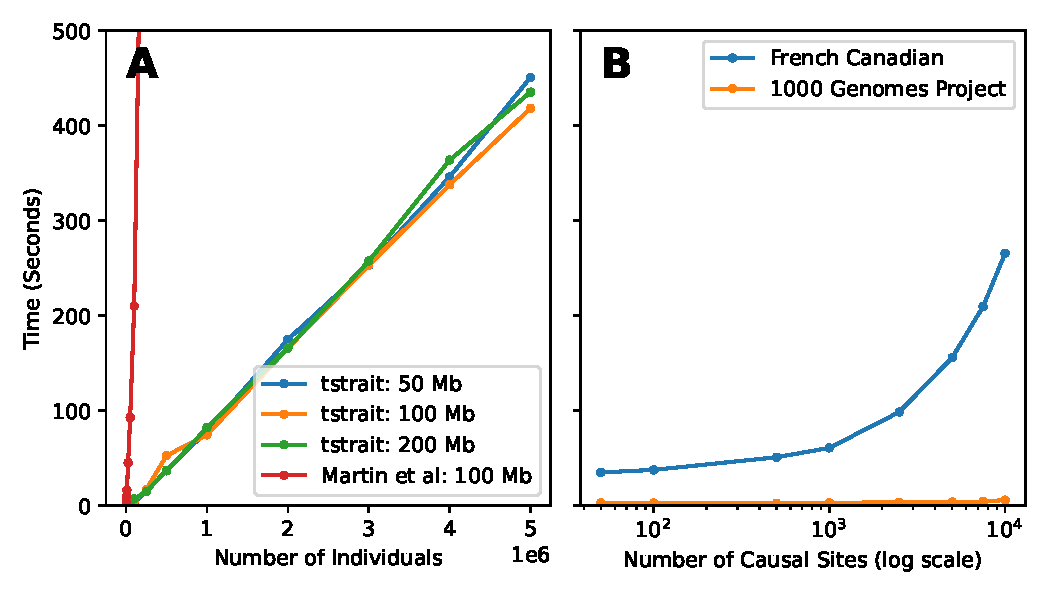
\includegraphics[width=213pt]{figures/time-scaling.pdf}
\caption{\textbf{Time taken to simulate quantitative traits.} Each point
represents the mean time for 10 independent runs under different random seeds.
The times reported are the total CPU time required to simulate quantitative
traits on an Intel(R) Core(TM) i9-11900H CPU and 16 GB of RAM. The trait model
is a normal distribution with $\mu=0$, $\sigma^2=1$, $h^2=0.3$, and
$\alpha=-1$. (A) Computational time with increasing number of individuals. The
whole genome dataset from \emph{Homo sapiens} with various number of
individuals and chromosome length are simulated by using \texttt{stdpopsim}
\citep{adrion2020}. For each replicate of the simulation, \texttt{tstrait} is
used to simulate one quantitative trait with 1000 causal sites. (B)
Computational time with increasing number of causal sites on two large
realistic ARGs. \texttt{tstrait} is used to simulate quantitative traits from
the simulated French Canadian dataset \citep{anderson2023} and the inferred
tree sequence dataset of the 1000 Genomes Project \citep{kelleher2019} with
varying number of causal sites. The French Canadian dataset is downloaded from
\url{https://zenodo.org/record/6839683}, and the inferred ARG from the 1000
Genomes Project is downloaded from \url{https://zenodo.org/record/3051855}.
Chromosome 9 is selected for both datasets.}\label{fig:time}
\end{figure}

\section{Conclusion}

We believe that in the coming years, simulation in tree sequence encoding will
attract more users in need of conducting genetic simulations with complex
population structure. Multiple studies highlight the advantages of using the
ARG data structure in GWAS \citep{link2023tree,nowbandegani2023extremely,zhang2023}.
ARG data
structure is becoming increasingly useful in genetic studies, as it is possible
to accurately infer biobank-scale genealogies from sequencing data
\citep{zhang2023}, and simulate large sample whole-genome sequences with
spatiotemporal metadata \citep{anderson2023}. These advances in ARG presents a
real opportunity for people to further understand the effects of complex
population structure on quantitative traits. The \texttt{tstrait} package is an
essential piece of infrastructure that lets people explore these possibilities.

\section{Competing interests}
No competing interest is declared.

\section{Acknowledgments}

We greatly acknowledge helpful discussions about quantitative trait simulation
with Gregor Gorjanc. We thank Ben Haller and people in the tskit community for
helpful discussions and feedback. We thank Ben Jeffery for his help with the
Python package development.

\section{Funding}

D.T. is supported by the Oxford Kobe Scholarship from the University of Oxford
and the Euretta J. Kellett Fellowship from Columbia University.

This work was supported by ...


%USE THE BELOW OPTIONS IN CASE YOU NEED AUTHOR YEAR FORMAT.
\bibliographystyle{abbrvnat}
\bibliography{paper}

\end{document}
